\section{Übersicht der Pipeline}


Abbildung \ref{fig:ml_pipeline} zeigt den Aufbau der typischen Pipeline, um ein Neuronales Netz zu trainieren. 
Diese wird im Folgenden genauer beschrieben.
Schritt 1 ist die Vorverarbeitung der Daten.
Die Daten können dabei aus einer Datenbank oder einem Filesystem stammen, die im Voraus gesammelt wurden.
Die Vorverarbeitung der Daten ist recht individuell und kann je nach Anwendungsfall variieren. 
Typische Handlungen sind:
\begin{compactitem}
\item Vereinheitlichung des Datenformats
\item Fehler und starke Ausreißer werden entfernt
\item Normalisierung der Daten
\item Erstellung neuer Daten durch Transformationen
\item Kodierung von (kategorialen) Variablen und Labels
\item Aufteilung in Trainings-, Validierungs- und Testdatensätze
\end{compactitem}
\begin{figure}[!htb]
    \centering
    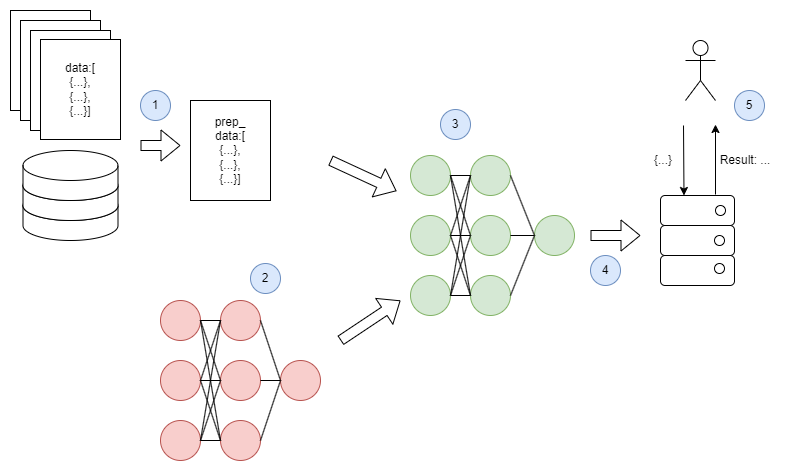
\includegraphics[width=14cm]{figures/ml_pipeline.png}
    \caption{Training eines Neuronalen Netzes}
    \label{fig:ml_pipeline}
\end{figure} 

Die Abbildung \ref{fig:ml_pipeline} stellt die Vorverarbeitung in einem Schritt dar, bei dem mehrere Datenquellen verbunden werden und nur ein Dokument übrig bleibt. 
Dieses eine Dokument soll zeigen, dass nur die wichtigen Informationen der Daten erhalten bleiben, jedoch kann es in der Praxis sein, dass die Datenmenge beim Aufbereiten der Daten größer wird. 
Kapitel \ref{sec:training_modells} stellt verschiedene Methoden vor, die bei der Vorverarbeitung der Daten angewendet werden können, um die Vertraulichkeit zu sichern.

Schritt 2 umfasst die Architektur eines Modells.
Je nach Anwendungsfall und Komplexität der Aufgabe, werden unterschiedliche Konfigurationen der einzelnen Schichten vorgenommen.
Dabei werden die Gewichte zufällig oder anhand einer Verteilung initialisiert.
In der Abbildung wird dies durch ein rotes Modell angezeigt, da Gewichte des Modell zufällig (oder anhand einer Verteilung) initialisiert sind, und noch keine sinnvolle Vorhersage getroffen werden kann.
Schritt 3 ist der tatsächliche Trainingsvorgang, bei dem das untrainierte Modell lernt.
Grob lässt sich das Training in folgende Schritte einteilen, die mehrfach mit jedem Datenpunkt durchgeführt werden können:
\begin{compactenum}
\item Ein Datenpunkt oder ein mehrere Datenpunkte (Batch) werden durch das Modell gegeben und die Vorhersage berechnet. Die Abweichung von der tatsächlichen Vorhersage zu dem Label des Datenpunktes wird mittels einer Verlustfunktion quantifiziert.
\item Mittels des Wertes der Verlustfunktion lassen sich Gradienten für die Gewichte des Neuronalen Netzes berechnen. Diese können dazu genutzt werden, die aktuellen Gewichte anzupassen. Dieser Schritt wird Backpropagation genannt.
\end{compactenum}
Ein Durchgang der obigen Schritte mit jedem Datenpunkt wird dabei Epoche genannt. 
Um den Trainingsfortschritt zu beobachten, kann eine Epoche zusätzlich auch eine Evaluierung mittels eines Validierungsdatensatzes enthalten.
Grafisch wird das Training durch den Verbund des Dokuments und des untrainierten, roten Modells dargestellt. 
Es entsteht ein grünes Modell, welches in der Lage ist, sinnvolle Vorhersagen zu erzeugen.
In der Praxis gibt es hier einige Iterationen des Training, welche zusätzliche Vorgänge, wie beispielsweise eine Validierung, enthalten. 
Kapitel \ref{sec:training_modells} widmet sich Methoden, die während des Trainings, welche aus Schritt 2 und 3 besteht, angewendet werden.

Schritt 4 und 5 beschreiben das Deployment und den Betrieb des Modells. 
Dieses soll für vorgesehene Anwender erreichbar sein. 
Je nach Anwendungsfall kann die Systemarchitektur unterschiedlich aussehen. 
Einige Modelle werden mit Trainingscode auf öffentlichen Plattformen, wie HuggingFace\footnote{https://huggingface.co/models}, geteilt, wohingegen andere Modelle, wie ChatGPT\footnote{https://chat.openai.com/}, nur über eine spezielle Oberfläche erreichbar sind.
In Abbildung \ref{fig:ml_pipeline} zeigt deshalb lediglich einen Anwender, der direkt Request an das Modell schickt.
In Kapitel \ref{sec:betrieb} werden Maßnahmen besprochen, die in dieser Phase die Vertraulichkeit sichern. 
Dabei kann es sich um Transformationen des Modells vor dem Deployment handeln, oder um Mechanismen, die Anfragen und Antworten des Modells abwandeln.